%% types
\newcommand{\fold}[2]{\let\@tmpop=\relax\@for\@I:=#2\do{\@tmpop\@I\let\@tmpop=#1}}
\newcommand{\record}[1]{\{\fold{,}{#1}\}}
\newcommand{\union}[1]{[\fold{,}{#1}]}
\newcommand{\sq}{\subseteq}

In this section, we describe the parts of the MitM ontology, which is a formal development in the MMT system.
The formalizations can be found at \url{https://gl.mathhub.info/MitM/}.
That location also contains various other archives in the \href{https://gl.mathhub.info/MitM/}{\texttt{MitM} library}, which are experiments, where the MitM ontology has been picked up by other projects.

The MitM ontology consists of two parts: the \textbf{MitM Foundation} which provides the logical language in which the mathematical domains in the MitM ontology can be described, and the \textbf{MitM Core}, which consists of the knowledge about these domains represented in the MitM foundation.

\subsection{The MitM Foundation}\label{sec:foundation}

The MitM foundation provides the type system and logic for the MitM ontology, i.e., the basic representational infrastructure used in the MitM ontology.
It is developed in the archive  \href{https://gl.mathhub.info/MitM/Foundation}{\texttt{Foundation}} (4 files, 539k LoF (lines
of formalization), 103 commits).

While the logic is relatively straightforward, the standardization of the type system was very difficult because mathematics requires a rich, open-ended type system, yet concrete implementations must stay as simple as possible.
After surveying the OpenDreamKit systems, we developed the types described in appendix~\ref{app:types}.

In a nutshell, the MitM foundation provides base types for all arithmetical number systems and common data structures like strings/words and Boolean values.
Complex types build on this include structural ones like (total and partial dependent) function, product, record, types, and mathematical constructions like sets, multisets, ists, vectors, and matrices.
In particular, dependent record types allow to represent types for mathematical structures (e.g. rings, fields, polynomials, finite maps, etc.) and their models.
These can also be constructed from OMDoc/MMT theories via the novel \textsf{Mod} operator~\cite{MueRabKoh:tat18}.

Finally, the MtiM foundation supports subtyping for the arithmetical number systems ($\mathbb{N}\subseteq\mathbb{Z}\subseteq\mathbb{Q}\subseteq\mathbb{R}\subseteq\mathbb{C}$), and along the sub-model relation.
This allows to express many mathematical identies very naturally.

\subsubsection{Expressions}

The MitM foundation allows the following \textbf{formulas}, i.e., expression of type $Boolean$:
\begin{itemize}
\item the propositional connectives: conjunction, disjunction, implication, negation, and equivalence of formulas as well as truth and falsity,
\item typed equality: $t\doteq_T t'$ for any two terms $t,t'$ of type $T$,
\item typed quantifiers: $\forall x:T.F(x)$ and $\exists x:T.F(x)$ for a type $T$ and a formula $F$,
\end{itemize}
Additionally, we allow shallow quantification over types: $\{a\}F(a)$ for a formula $F$ and a type variable $a$ is a formula but it may not --- to avoid inconsistency issues --- occur as a subformula of any of the above formula constructors.

We do not give the remaining straightforward \textbf{term} constructors in detail and only remark on a few important aspects.
Most critically, we allow types to have multiple representations that are semantically
equivalent but practically different in meaningful ways (e.g., because converting between
representations is expensive or imprecise). Moreover, some types have multiple constructors similar to an inductive type. In the sequel, we describe which representations are supported in those cases.

\paragraph{Integers Modulo}
The elements of $Z(m)$ are represented by $0,\ldots,m-1$.

\paragraph{Real Numbers}
A real number can be one of the following:
\begin{compactitem}
 \item a rational number
 \item an IEEE double precision float
 \item a root $\sqrt[n]{x}$ for $n\in N$ and $x\in Z$
 \item the strings "pi" and "e"
\end{compactitem}

\paragraph{Complex Numbers}
A complex number can be one of the following:
\begin{compactitem}
 \item Cartesian form $x+yi$
 \item polar form $r e^{i\phi}$
 \item root of unity $\zeta_n$
\end{compactitem}

\paragraph{p-Adic Numbers}
A $p$-adic number $x$ consists of unit $u\in N$ ($u,p$ co-prime), valuation $v\in Z$, and precision $r\in N$ (for $u<p^r$).

\paragraph{Polynomials}
For $r\in Ring$ and distinct strings $x_i$, we consider polynomials
\[p\in Polynomial(r,[x_1,\ldots,x_n])\]
to be of the form $p=\Sigma_{\vec{i}\in N^n} a_{\vec{i}} \vec{x}^{\vec{i}}$ where and $(x_1,\ldots,x^n)^{(i_1,\ldots,i_n)}$ abbreviates $x_1^{i_1}\cdot \ldots\cdot x_n^{i_n}$.

\paragraph{Rings}
A ring can be one of the following:
\begin{compactitem}
 \item a field
 \item $Polynomial(r,[x_1,\ldots,x_n])$ for $r\in Ring$
\end{compactitem}

\paragraph{Fields}
A field can be one of the following:
\begin{compactitem}
 \item base fields $Q$, $R$, and $C$
 \item finite fields $Z(p)$ for $p\in Prime$ (same type as integers modulo $p$)
 \item polynomial field extensions $FieldExtension(F,p,a)$ of $F\in Field$ for a polynomial $p\in Polynomial(F,[x])$ (for any variable name $x$)
 \item named fields identified by a string
\end{compactitem}

We define some abbreviations for common fields:
\begin{compactitem}
 \item $Q(p,a)=FieldExtension(Q,p,a)$
 \item $Qsqrt(n,a)=Q(x^2-n,a)$
 \item $Qzeta(n,a)=Q(y_n,a)$ where $y_n$ is the $n$-th cyclotomic polynomial
\end{compactitem}

We do not define $GF(q)$ for $q=p^n$ as an abbreviation for $FieldExtension(Z(p),g)$ for some irreducible polynomial $g\in Polynomial(Z(p))$ of degree $n$ because there is no way to choose $g$ canonically and it is necessary to know $g$ to represent the elements of $GF(q)$.

\paragraph{Structure Elements}
Every structure has an underlying type, which is used to represent its elements.

The underlying types of fields are defined as follows:
For $Q$, $R$, $C$, and $Z(p)$, the underlying type is the field itself.
The underlying type of $FieldExtension(F,p,a)$ is $Polynomial(F,[a])$ ($a=x$ is allowed).

% % % % % % % % % % % % % % % % % % % % % % % % % % % % %
\subsection{MitM Core}

The \textbf{MitM core} in the
  \href{https://gl.mathhub.info/MitM/smglom}{\texttt{smglom}}\footnote{The name
    \texttt{smglom} was initially chosen for the ``Semantic Multilingual Glossary of
    Mathematics'' (SMGloM; see \ref{sec:smglom} below) with which it is
    cross-referenced. We will rethink naming once the MitM Ontology stabilizes.}  archive
  (43 files, 2600 LoF, 370 commits). It carries the bulk of the knowledge representation in
  the MitM Ontology. The main thrust of curation has been to get the VRE use cases
  reported on in~\cite{ODK-D6.5}, but we also have elementary formalizations of algebra,
  arithmetics, calculus, category theory, set collections, elliptic curves (for LMFDB),
  functional analysis, geometry, graph theory, measure theory, set theory, and topology.


In the sequel, we describe two exemplary parts of the MitM core ontology.

\subsubsection{Computational Group Theory}

\ednote{specify file name and size of the ontology}
Our formalization of CGT follows the template of its implementation in \GAP, and requires several levels of abstraction -- currently \emph{abstract}, \emph{representation}, \emph{implementation}, and \emph{concrete}. From our experience, we expect this pattern to be applicable across computational algebra, possibly with additional levels of abstraction. 
The left box in Figure \ref{fig:cgtontology} gives an overview.

The abstract level contains the axioms and basic definitions of the theory of \emph{Groups}: generating sets, homomorphisms, group actions, stabilisers, and orbits.
The most basic part is given in Figure~\ref{fig:mitm1}. 
\begin{figure}[ht]\centering
  \fbox{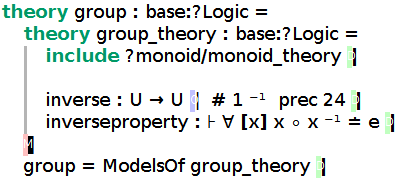
\includegraphics[width=8cm]{../MACIS17-interop/mitm1}}
  \caption{A Formalization of a Group}\label{fig:mitm1}
\end{figure}

At the representation level groups are described as concrete objects
suitable for computations: groups of permutations, groups of matrices,
finitely presented groups, groups obtained by algebraic constructions or using
polycyclic presentations.

At the implementation level, we encode implementation details: for
example, permutation groups are considered as finite subgroups of the group $S_{\mathbb{N}+}$, and defined \ednote{constructed?} by
providing a set of generating permutations.

At the concrete level, the computation happens: while the higher levels
are suitable for mathematical deduction and inference, this level is where OpenDreamKit systems like \GAP perform their main work.

\subsubsection{Modeling and Simulation}

The \href{https://gl.mathhub.info/MitM/smglom}{\texttt{models}}
archive (11 files, 650 LoF, 113 commits) is an experimental extension
of the MitM ontology, where we test the expressive power of MitM
framework (and the OpenDreamKit technologies) by applying it to a
field well outside of mathematics, namely for modeling and simulation
in opto-electronics.

%%% Local Variables:
%%% mode: visual-line
%%% fill-column: 5000
%%% mode: latex
%%% TeX-master: "report"
%%% End:

%  LocalWords:  formalizations texttt formalization standardization subsubsection textbf newcommand subseteq textsf MueRabKoh:tat18
%  LocalWords:  compactitem ednote adic ldots,a_n ldots,a_n ldots,T_n ldots Vec monoid sq
%  LocalWords:  FiniteHybridset subtyping emph leq_T leq_ leq_ leq_ r,x s,y leq doteq_T
%  LocalWords:  t,t forall subformula u,p ldots,x cdot cdot Qsqrt Qzeta th smglom fbox
%  LocalWords:  stabilizes fig:cgtontology fig:mitm1 centering includegraphics mathbb
